\documentclass[UTF-8,twoside,cs4size]{ctexart}
\usepackage[dvipsnames]{xcolor}
\usepackage{amsmath}
\usepackage{amssymb}
\usepackage{geometry}
\usepackage{listings}
\usepackage{setspace}
\usepackage{xeCJK}
\usepackage{ulem}
\usepackage{pstricks}
\usepackage{pstricks-add}
\usepackage{bm}
\usepackage{mathtools}
\usepackage{breqn}
\usepackage{mathrsfs}
\usepackage{esint}
\usepackage{textcomp}
\usepackage{upgreek}
\usepackage{pifont}
\usepackage{tikz}
\usepackage{circuitikz}
\usepackage{caption}
\usepackage{tabularx}
\usepackage{array}
\usepackage{pgfplots}
\usepackage{multirow}
\usepackage{pgfplotstable}
\usepackage{mhchem}
\usepackage{graphicx}
\usepackage[cache=false]{minted}

\newcolumntype{Y}{>{\centering\arraybackslash}X}
\geometry{a4paper,centering,top=1.27cm,bottom=2.54cm,left=2cm,right=2cm}
\graphicspath{{figures/}}
\pagestyle{plain}
\captionsetup{font=small}

%\CTEXsetup[name={,.}]{section}
\CTEXsetup[format={\raggedright\heiti\noindent\zihao{3}},numberformat={\bfseries}]{section}
\CTEXsetup[format={\raggedright\heiti\zihao{-3}},numberformat={\bfseries}]{subsection}
\CTEXsetup[format={\raggedright\heiti\quad\zihao{4}},numberformat={\bfseries}]{subsubsection}
\CTEXsetup[format={\raggedright\heiti\qquad},numberformat={\bfseries}]{paragraph}
\CTEXsetup[beforeskip=1.0ex plus 0.2ex minus .2ex, afterskip=1.0ex plus 0.2ex minus .2ex]{paragraph}

\CTEXsetup[format={\raggedright\heiti\qquad},numberformat={\bfseries},name={\bfseries(,)}]{subparagraph}
\CTEXsetup[beforeskip=1.0ex plus 0.2ex minus .2ex, afterskip=1.0ex plus 0.2ex minus .2ex]{subparagraph}
\renewcommand\thefootnote{\ding{\numexpr171+\value{footnote}}}

\setstretch{1.5}

\setCJKfamilyfont{boldsong}[AutoFakeBold = {2.17}]{SimSun}
\newcommand*{\boldsong}{\CJKfamily{boldsong}}
%\DeclareMathOperator\dif{d\!}
\newcommand*{\me}{\mathop{}\!\mathrm{e}}
\newcommand*{\mpar}{\mathop{}\!\partial}
\newcommand*{\dif}{\mathop{}\!\mathrm{d}}
\newcommand*{\tab}{\indent}
\newcommand*{\mcelsius}{\mathop{}\!{^\circ}\mathrm{C}}
\renewcommand*{\Im}{\mathrm{Im}\,}

\setcounter{secnumdepth}{5}

\renewcommand\arraystretch{1.5}
\renewcommand\thesubparagraph{\arabic{subparagraph}}

\setminted{style=manni,fontsize=\small,breaklines=true}

\lstset{
	backgroundcolor=\color[RGB]{245,245,245},
	keywordstyle=\color{blue}\bfseries,
	basicstyle=\small\ttfamily,
	commentstyle=\itshape\color{olive},
	numberstyle=\ttfamily,
	tabsize=4,
	breaklines=true
}

\begin{document}
	\begin{center}
		\heiti\zihao{-2}
		实验\textbf{8 $ \bm\sim $ 9}报告
	\end{center}

	\begin{table*}[!h]
		\raggedleft
		\zihao{-4}
		\begin{tabular}{ccc}
			{\heiti 学号} & {2019K8009929019} & {2019K8009929026} \\
			{\heiti 姓名} & 桂庭辉 & 高梓源 \\
			{\heiti 箱子号} & \multicolumn{2}{c}{44}
		\end{tabular}
	\end{table*}
	
	\section{实验任务}
	
	截至Lab07,我们在五级静态流水线框架上迭代增加的指令均为用户态指令,本次实验添加部分内核态功能,基于LoongArch 32位精简版指令系统支持部分异常与中断的处理。
    
    Lab08以系统调用异常(由\texttt{syscall}指令触发)为引,引入CSR实现以及已有流水线与CSR的交互,构建异常处理的基本框架。
    
    Lab09在Lab08的基础上添加部分异常检测逻辑,并实现时钟中断。
	
	\section{实验设计}
    \subsection{总体设计思路}
    
    CSR的内部实现主要参考实验讲义,后续不再详述该部分逻辑。在流水线中引入与CSR的交互需确定其读写逻辑所处的流水级。考虑\texttt{csrwr}与\texttt{csrxchg}指令“交换”通用寄存器与控制状态寄存器的值,将CSR数据在流水线中的行为与通用寄存器尽可能一致化,在ID级异步读CSR,在WB级同步写CSR。后续将进一步讨论该方案中数据相关的处理与实际性能表现。
    
    本次实验共添加\texttt{syscall, csrrd, csrwr, csrxchg, break, rdcntid.w, rdcntvl.w, rdcntvh.w}共8条指令,其译码逻辑不再赘述,根据具体功能在下文分别介绍其功能实现。
    
    在本次实验的测试中,由软件事先设置异常处理程序入口,即EENTRY寄存器记录的地址。指令沿流水线逐级检测并记录异常信息,当发生异常的指令流到写回级时,拉高异常发生信号\texttt{wb\_exc},将该指令的PC值写入ERA寄存器,关闭中断使能,更新ESTAT等寄存器,清空流水线跳转至异常处理程序入口。此后执行异常处理程序直至\texttt{ertn}指令退出异常处理程序,当\texttt{ertn}流至写回级时,拉高\texttt{wb\_ertn},清空流水线,跳转至ERA寄存器记录PC,更新中断使能等CSR信息。
    
    \subsection{流水线的清空与精确异常}
    在Lab08与Lab09中我们采用了两种不同的形式进行流水线清空。
    
    在Lab08中,我们参考Lab03、04解决控制相关的思路,通过对流水级的\texttt{valid}信号同步置0来取消即将进入当前流水级的指令。以执行级为例,代码实现如下:
    
    \begin{minted}{verilog}
    always @(posedge clk) begin
        if (reset) begin
            es_valid <= 1'b0;
        end else if (wb_exc | wb_ertn) begin
            es_valid <= 1'b0;
        end else if (es_allowin) begin
            es_valid <= ds_to_es_valid;
        end
    end
    \end{minted}
    
    容易发现,如果对五级流水均采用上述形式清空流水线,将会在流水线首部的取指级、尾部的写回级出现一些问题。
    
    当异常发生信号\texttt{wb\_exc}或异常返回信号\texttt{wb\_ertn}被拉高时,位于写回级的指令并没有一个将要进入的流水级,也就无从被取消,但可以通过取消其寄存器堆写使能与CSR写使能来取消该指令的行为产生效果,从而实现精确异常。
    
    本次实验中另一处精确异常实现要点为store指令,其产生效果并非如其他指令在写回级,而是在执行级对数据SRAM发使能。故而当其需要被刷掉,即执行、访存、写回级上有异常信号或\texttt{ertn}指令时,需要强制取消其数据RAM字节写使能。
    
    \begin{minted}{verilog}
    assign store_cancel = wb_exc | wb_ertn | ms_to_es_st_cancel | (|es_exc_flgs);
    
    assign data_sram_wen = store_cancel ? 4'h0                               :
                         es_store_op[2] ? (4'h1 <<  es_alu_result[1:0])      : // b
                         es_store_op[1] ? (4'h3 << {es_alu_result[1], 1'b0}) : // h
                         es_store_op[0] ? 4'hf : 4'h0;                         // w
    \end{minted}
    
    回到此前提到的当前清空流水线对取指的影响上来,当对\texttt{fs\_valid}同步置0时,应当如何设置或生成正确的\texttt{nextpc}?如果异步地修改\texttt{nextpc},那么下一拍指令进入IF级时\texttt{fs\_valid}为0,该指令会被错误地取消。观察\texttt{fs\_valid}置0后的流水线状态,可注意到此时所有流水级均被清空,流水线等效于未启动。由此可以想到,可以参考复位释放前\texttt{fs\_pc}的设置,即设置为$ \text{初始PC}-4 $,在刷新流水线时将\texttt{fs\_pc}同步置为$ \mathrm{exc\_entry}\text{或}\mathrm{exc\_retaddr}-4 $,流水线即可从异常处理入口或返回地址“重新启动”。
    
    \begin{minted}{verilog}
always @(posedge clk) begin
    if (reset) begin
        fs_pc <= 32'h1bfffffc;
    end else if (wb_exc | wb_ertn) begin
        fs_pc <= (wb_exc ? exc_entry : exc_retaddr) - 32'h4;
    end else if (to_fs_valid && fs_allowin) begin
        fs_pc <= nextpc;
    end
end
    \end{minted}
    
    回顾上述过程的时序,可以注意到每次进入与退出异常处理程序时均会浪费1拍,那么有没有基于异步的流水线清法可以避免这样的性能损失呢?\footnote{当然,此处并非性能热点,经过测试,在当前测试程序与时钟频率下,对该处优化的收益仅为1720\,ns。此外,基于已有的同步清法,可以不将\texttt{fs\_valid}同步置0,简单异步修改流水线控制信号即可避免浪费,此处讨论一种全异步的清法来进一步了解流水线时序。}
    
    此处清空流水线的工作最终目的是在\texttt{wb\_exc}或\texttt{wb\_ertn}(下文以“流水线刷新使能”称呼二者)拉高的下一拍获得一个IF级为异常入口或返回地址指令、其他流水级无效的流水线状态。流水线状态的更新发生在这个“下一拍”的刷新处,那么在流水线刷新使能拉高的周期内异步地准备好流水线状态即可。基于上述想法,具体实现上分为两个部分,其一是将除pre-IF外的每个流水级传递给下游流水级的\texttt{valid}信号置0,其二是将被阻塞的流水级释放阻塞,确保流水线状态更新的发生。以译码级为例,代码实现如下:
    
    \begin{minted}{verilog}
assign ds_ready_go    = ~(es_blk | csr_blk) | (wb_exc | wb_ertn);
assign ds_to_es_valid = ds_valid & ds_ready_go & ~(wb_exc | wb_ertn);
    \end{minted}
    
    \subsection{\textbf{CSR}读写拆分与数据相关}
    
    出于对\texttt{csrwr, csrxchg}指令中通用寄存器与控制状态寄存器数据“交换”这一行为的考虑,我们在ID级异步读CSR,WB级同步写CSR,使得CSR寄存器数据行为与通用寄存器尽可能一致。此外CSR写的相关信号,如写使能、写寄存器号、写掩码、写数据均在ID级生成,依次传递至后续流水级。
    
    这样拆分自然导致CSR的写后读数据相关,其中一部分与通用寄存器的RAW相关类似,由不同的CSR读写指令对同一CSR寄存器先写后读。另一部分来自部分通用寄存器的特殊用途,具体参见实验讲义6.3.4节。此处对于CSR数据相关均采用阻塞方式解决。
    \begin{minted}{verilog}
assign {es_csr_we, es_eret, es_csr_wnum} = es_csr_blk_bus;
assign {ms_csr_we, ms_eret, ms_csr_wnum} = ms_csr_blk_bus;
assign {ws_csr_we, ws_eret, ws_csr_wnum} = ws_csr_blk_bus;

assign csr_blk = ds_csr_re & (es_csr_blk | ms_csr_blk | ws_csr_blk);
assign es_csr_blk = es_csr_we &&  csr_rnum == es_csr_wnum && es_csr_wnum != 0 ||
                    es_eret   &&  csr_rnum == `CSR_CRMD                       ||
                    inst_ertn && (es_csr_wnum == `CSR_ERA || es_csr_wnum == `CSR_PRMD);
assign ms_csr_blk = ms_csr_we &&  csr_rnum == ms_csr_wnum && ms_csr_wnum != 0 ||
                    ms_eret   &&  csr_rnum == `CSR_CRMD                       ||
                    inst_ertn && (ms_csr_wnum == `CSR_ERA || ms_csr_wnum == `CSR_PRMD);
assign ws_csr_blk = ws_csr_we &&  csr_rnum == ws_csr_wnum && ws_csr_wnum != 0 ||
                    ws_eret   &&  csr_rnum == `CSR_CRMD                       ||
                    inst_ertn && (ws_csr_wnum == `CSR_ERA || ws_csr_wnum == `CSR_PRMD);
    \end{minted}
    
    当然,也可以将CSR的读写均放在WB级进行,这样CSR不会发生数据相关,但需要注意的是csr指令需在写回级才能拿到数据,相应地需要将与其产生通用寄存器RAW相关的ID级阻塞至csr指令完成。该方案实现较为简单,此处省略代码实现。
    
    对比以上二者性能,其他条件一致时,在Lab09的测试下,拆分读写仿真用时1785555\,ns,均在WB级完成用时1793595\,ns。分析其原因,将CSR数据取到通用寄存器后通常要对通用寄存器进行维护以间接维护CSR,故而在后者情况下引发数据相关导致阻塞的次数更多。
    
    当然,同此前讨论流水线清空时的性能问题一样,此处同样不是程序热点,对整体性能的影响不到1\%。
    
    \subsection{异常检测、时钟中断与计时器}
    目前需支持的6种异常中,一种(ADEF)由取指级标记,四种由译码级标记,其中两种(SYS、BRK)来自特定指令,一种为中断INT,一种(INE)来自所有指令译码结果取反,最后一种异常(ALE)由执行级标记。
    
    SYS、BRK、INE由译码结果可自然得到,INT由CSR模块的维护也可自然得到,ADEF、ALE对取指或访存地址的低位进行相应判断即可。
    
    需要注意的是,异常之间存在优先级关系,中断$ > $取指级标记异常$ > $译码级标记异常$ > $执行级标记异常,在ecode的生成逻辑中需要有所体现。
    \begin{minted}{verilog}
assign wb_ecode    = ws_exc_flgs[`EXC_FLG_INT ] ? `ECODE_INT :
                     ws_exc_flgs[`EXC_FLG_ADEF] ? `ECODE_ADE :
                     ws_exc_flgs[`EXC_FLG_INE ] ? `ECODE_INE :
                     ws_exc_flgs[`EXC_FLG_SYS ] ? `ECODE_SYS :
                     ws_exc_flgs[`EXC_FLG_BRK ] ? `ECODE_BRK :
                     ws_exc_flgs[`EXC_FLG_ALE ] ? `ECODE_ALE : 6'h00;
assign wb_esubcode = {9{ws_exc_flgs[`EXC_FLG_ADEF]}} & `ESUBCODE_ADEF;
    \end{minted}
    
    对于ALE,需要记录并传递错误的访存地址,具体实现上我们复用原有流水槽中记录指令寄存器堆写数据的部分进行传递。
    
	时钟中断的实现参考实验讲义对相关控制寄存器进行维护即可。
    
    三条计时器相关指令中,\texttt{rdcntid.w}功能类似\texttt{csrrd},类似处理即可,\texttt{rdcntvl.w}与\texttt{rdcntvh.w}需要访问一个独立的64位计时器,在流水槽中添加其使能\texttt{rdcn\_en}与高低位选择\texttt{rdcn\_sel}信号,在适当流水级\footnote{由于自行设计的除法器时序较差,若在执行级取计时器值与ALU结果合并,则会导致整体时序违约,故而我们选择暂时将计时器的读取放在访存级。}读取计时器值即可。
    
    \begin{minted}{verilog}
assign ms_final_result = ms_rdcn_en ? stable_cnter[{ms_rdcn_sel, 5'b0}+:32] :
                         ms_exc_flgs[`EXC_FLG_ALE] ? ms_alu_result :
                         ms_res_from_mul           ? mul_result    :
                         (|ms_load_op)             ? load_result   :
                                                     ms_alu_result;

always @ (posedge clk) begin
    if (reset) begin
        stable_cnter <= 64'b0;
    end else begin
        stable_cnter <= stable_cnter + 64'b1;
    end
end
    \end{minted}
    
	\section{实验过程}
	\subsection{实验流水账}
	
	\noindent2021.10.15 20:00 $\sim$ 2021.10.16 00:00:完成Lab08
    
    \noindent2021.10.20 15:00 $\sim$ 2021.10.20 18:00:完成Lab09
    
    \noindent2021.10.24 20:00 $\sim$ 2021.10.24 23:00:尝试并测试不同的流水线清空、CSR读写规划策略
    
    \noindent2021.10.25 18:00 $\sim$ 2021.10.25 22:00:撰写实验报告
	
	\subsection{错误记录}
    \subsubsection{错误\textbf{1:}基础逻辑关系错误}
    \paragraph{错误现象}\hfill
    
    编写完Lab08代码后仿真运行发现未能正确发生阻塞。
    
    \paragraph{分析定位过程}\hfill
    
    观察相关指令波形,注意到如下情形:
    \begin{figure}[!h]
        \centering
        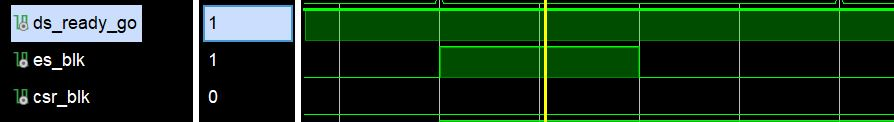
\includegraphics[width=0.8\textwidth]{08-dbg-01.jpg}
        \caption{阻塞逻辑错误}
    \end{figure}
        
    \paragraph{错误原因}\hfill
    
    由\texttt{es\_blk}、\texttt{csr\_blk}生成\texttt{ds\_ready\_go}的逻辑错误。
    
    \paragraph{修正效果}\hfill
    
    重新梳理逻辑关系,修订代码如下:
    \begin{minted}{verilog}
    assign ds_ready_go = ~(es_blk | csr_blk) | (wb_exc | wb_ertn);
    \end{minted}
	
    \paragraph{归纳总结}\hfill
    
    该类错误来自于代码编写时未仔细考量逻辑关系,属于低级错误,下文不再讨论该类基础逻辑错误与笔误。
    
    \subsubsection{错误\textbf{2:}同步清空流水线跳转错误}
    \paragraph{错误现象}\hfill
    
    使用前文介绍的全同步清空流水线策略时,异常处理入口处\texttt{0x1c008000}的指令未被提交。
    
    \paragraph{分析定位过程}\hfill
    
    考察IF级在异常发生前后的波形特点,注意到\texttt{0x1c008000}处指令进入IF级恰好\texttt{fs\_valid}为0,该指令被取消。
    
    \paragraph{错误原因}\hfill
    
    未充分审视梳理所用流水线清空策略下的时序关系,异步地修改\texttt{nextpc}导致入口处指令下一拍进入IF级时正好被取消。
    
    \paragraph{修正效果}\hfill
    
    重新梳理时序关系,以上文介绍的模仿复位释放过程同步设置\texttt{fs\_pc}方式让流水线在异常处理入口处重新启动。此后正常完成异常处理的跳转操作。
    
    \subsubsection{错误\textbf{3:}异步清空流水线被阻塞}
    \paragraph{错误现象}\hfill
    
    使用前文介绍的全异步清空流水线策略时,异常处理跳转失败,指令仍按原次序提交。
    
    \paragraph{分析定位过程}\hfill
    
    观察IF级、ID级在异常发生前后的波形,注意到异常处理入口\texttt{0x1c008000}正确进入IF级,但由于ID级恰好发生通用寄存器阻塞占用流水级,导致流水线状态更新失败,进而舍弃此时IF级的指令。
    
    \paragraph{错误原因}\hfill
    
    未考虑阻塞发生时的流水线更新特征,进而未强制释放阻塞指令,导致流水线未能清空,异常处理入口也不能正常进入流水线。
    
    \paragraph{修正效果}\hfill
    
    如前文所述添加相应逻辑强制释放被阻塞的流水级,正常进行异常处理的跳转操作。
    
    \paragraph{归纳总结}\hfill
    
    2、3两个错误为时序问题,在设计方案时考虑不够充分,完成主要逻辑的同时未能兼顾细节上的维护。
	\section{实验总结}
    
    本次实验中我们尝试了不同方式实现同一功能,对流水线有了更深刻的体会,也直观地注意到设计方案对性能的影响。
    
    由于Lab06中除法器延时过高的遗留问题,本次实验中在最长路径(ALU $\to$ 前递选择 $\to$ \texttt{nextpc})上几乎不能添加额外的内容,如64位恒定频率计时器就被迫移到访存级访问。由于期中与其他课程压力等原因,本次未能修订除法器延时的问题,希望在下面两次实验中能够及时予以修订。
\end{document}